% Source-backed analysis update assembled from:
%   ../docs/ml_results.md
%   ../docs/progress.md
%   ../docs/roadmap.md
%   ../Analysis_CODES/docs/ppref_x_reweighted_working_points.md
%   ../Analysis_CODES/docs/pbpb24_psi2s_selection_mass_scan.md
\documentclass[11pt,aspectratio=169]{beamer}

\usetheme{Madrid}
\usecolortheme{default}
\setbeamertemplate{navigation symbols}{}
\setbeamertemplate{footline}[frame number]

\usepackage{booktabs}
\usepackage{graphicx}
\usepackage{tikz}
\usetikzlibrary{arrows.meta,positioning}
\input{beamer_setup.tex}

\definecolor{positive}{HTML}{0173B2}
\definecolor{negative}{HTML}{DE8F05}
\definecolor{emphasis}{HTML}{027A5A}
\definecolor{neutral}{HTML}{666666}
\definecolor{panelbg}{HTML}{F4F6F8}
\setbeamercolor{structure}{fg=positive}
\setbeamercolor{block title}{fg=white,bg=positive}
\setbeamercolor{block body}{fg=black,bg=positive!8}
\setbeamercolor{block title alerted}{fg=white,bg=negative}
\setbeamercolor{block body alerted}{fg=black,bg=negative!10}
\setbeamercolor{block title example}{fg=white,bg=emphasis}
\setbeamercolor{block body example}{fg=black,bg=emphasis!8}
\newcommand{\pos}[1]{\textcolor{positive}{#1}}
\newcommand{\con}[1]{\textcolor{negative}{#1}}
\newcommand{\HL}[1]{\textcolor{emphasis}{#1}}
\newcommand{\muted}[1]{\textcolor{neutral}{#1}}

\title[X(3872) Analysis Update]{X(3872) Analysis Update}
\subtitle{From \texorpdfstring{\psiP}{psi(2S)} reweighting to the current PbPb strategy}
\author{Lekai Yao}
\institute{CMS}
\date{2026.7.29}

\begin{document}

\begin{frame}[plain]
  \titlepage
  \vspace{-0.6em}
  \begin{center}
    \small ppRef prototype completed --- PbPb selection and fit diagnostics in progress
  \end{center}
\end{frame}

\begin{frame}{Analysis path: validate the chain, then move to PbPb}
  \centering
  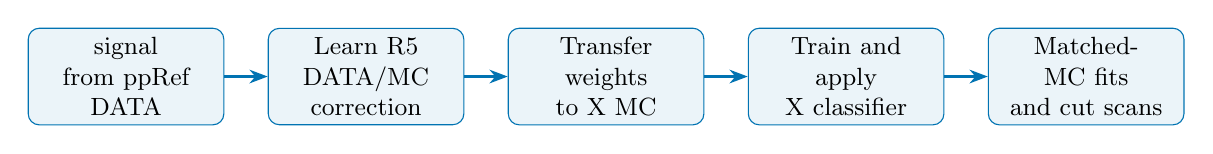
\begin{tikzpicture}[
    node distance=0.55cm,
    box/.style={
      draw=positive,
      rounded corners,
      fill=positive!8,
      minimum height=0.82cm,
      text width=2.25cm,
      align=center,
      font=\small
    },
    arrow/.style={-{Stealth},thick,positive}
  ]
    \node[box] (signal) {\psiP signal\\from ppRef DATA};
    \node[box,right=of signal] (rw) {Learn R5\\DATA/MC correction};
    \node[box,right=of rw] (apply) {Transfer weights\\to X MC};
    \node[box,right=of apply] (ml) {Train and apply\\X classifier};
    \node[box,right=of ml] (fit) {Matched-MC fits\\and cut scans};
    \draw[arrow] (signal) -- (rw);
    \draw[arrow] (rw) -- (apply);
    \draw[arrow] (apply) -- (ml);
    \draw[arrow] (ml) -- (fit);
  \end{tikzpicture}

  \vspace{1.0em}
  \begin{columns}[T]
    \begin{column}{0.48\textwidth}
      \begin{block}{ppRef question}
        Can the complete correction $\rightarrow$ ML $\rightarrow$ fit workflow be validated?
      \end{block}
    \end{column}
    \begin{column}{0.48\textwidth}
      \begin{alertblock}{Interpretation boundary}
        Observed significance alone does not establish the final training preference.
      \end{alertblock}
    \end{column}
  \end{columns}
  \vfill
  \centering\small\HL{The ppRef prototype is now closed; the next bottleneck is PbPb \psiP.}
\end{frame}

\begin{frame}{ppRef \texorpdfstring{\psiP}{psi(2S)} reweighting: R5 nominal}
  \begin{columns}[T]
    \begin{column}{0.40\textwidth}
      \begin{block}{R5 inputs}
        \begin{itemize}
          \item \texttt{Bcos\_dtheta}
          \item \texttt{Btktkpt}
          \item \texttt{Bchi2Prob}
          \item \texttt{Btrk1Pt}, \texttt{Btrk2Pt}
        \end{itemize}
      \end{block}
      \vspace{0.3em}
      \begin{itemize}
        \item sWeighted \psiP DATA target
        \item Folded train/apply workflow
        \item R3/R4\_noCos retained as checks
        \item R8 excluded after comparison
      \end{itemize}
    \end{column}
    \begin{column}{0.57\textwidth}
      \centering
      \includegraphics[width=\textwidth,height=0.68\textheight,keepaspectratio]
      {../XGBoost/output/reweighting/comparison_pp24_psi2s/weight_distributions_R3_R4_R5_R8.pdf}
    \end{column}
  \end{columns}
  \vfill
  \centering\small
  Source: \texttt{docs/ml\_results.md}; R5 is the nominal ppRef prototype.
\end{frame}

\begin{frame}{Closure: little residual DATA/MC separation}
  \begin{columns}[T]
    \begin{column}{0.52\textwidth}
      \centering
      \includegraphics[width=\textwidth,height=0.60\textheight,keepaspectratio]
      {../XGBoost/output/reweighting/comparison_pp24_psi2s/domain_auc_stability.pdf}
    \end{column}
    \begin{column}{0.45\textwidth}
      \begin{exampleblock}{Independent holdout test}
        Domain-classifier AUC $\simeq \HL{0.5225}$, stable over five random splits.
      \end{exampleblock}
      \begin{itemize}
        \item Weight statistics validated
        \item X MC support/coverage checked
        \item \texttt{Reweight} written to X MC
        \item No obvious residual separation
      \end{itemize}
    \end{column}
  \end{columns}
  \vfill
  \centering\small\HL{R5 passes the ppRef closure and transfer checks used in this prototype.}
\end{frame}

\begin{frame}{X classifier: unweighted and R5-weighted 8v2}
  \begin{columns}[T]
    \begin{column}{0.49\textwidth}
      \centering
      \textbf{Unweighted X MC}\\[-0.1em]
      \includegraphics[width=\textwidth,height=0.58\textheight,keepaspectratio]
      {../XGBoost/output/training/X_pp24_v4_fid3_8v2_rw0_xgb_v1/roc.pdf}
      \scriptsize
      \texttt{X\_pp24\_v4\_fid3\_8v2\_rw0\_xgb\_v1}
    \end{column}
    \begin{column}{0.49\textwidth}
      \centering
      \textbf{R5-weighted X MC}\\[-0.1em]
      \includegraphics[width=\textwidth,height=0.58\textheight,keepaspectratio]
      {../XGBoost/output/training/X_pp24_v4_fid3_8v2_rwpsi2sr5v1_xgb_v1/roc.pdf}
      \scriptsize
      \texttt{X\_pp24\_v4\_fid3\_8v2\_rwpsi2sr5v1\_xgb\_v1}
    \end{column}
  \end{columns}
  \vfill
  \centering\small
  Both train/apply/draw chains and scored DATA/MC ROOT files are complete.
\end{frame}

\begin{frame}{Matched-MC working points}
  \vspace{4pt}
  \begin{center}
    \small
    \begin{tabular}{llrrrr}
      \toprule
      Training & Bkg. eff. & Status & Yield & Signif. & Mass [GeV] \\
      \midrule
      rw0 & 10\% & 0/0 & $762\pm63$ & 12.18 & 3.87028 \\
      rw0 & 3\%  & $-1$/3 & $286\pm80$ & 8.04 & 3.86884 \\
      rw0 & 1\%  & 0/0 & $112\pm20$ & 5.52 & 3.86703 \\
      \midrule
      R5 & 10\% & 0/0 & $775\pm65$ & 12.21 & 3.87174 \\
      R5 & 3\%  & 0/0 & $216\pm54$ & 5.84 & 3.87229 \\
      R5 & 1\%  & 0/0 & $78\pm23$ & 3.40 & 3.87208 \\
      \bottomrule
    \end{tabular}
  \end{center}
  \vspace{0.3em}
  \begin{columns}[T]
    \begin{column}{0.48\textwidth}
      \begin{block}{Interface fixed}
        Each training uses its own scored DATA and matched MC template.
      \end{block}
    \end{column}
    \begin{column}{0.48\textwidth}
      \begin{alertblock}{Comparison caveat}
        rw0 3\% did not converge; it cannot support a quantitative ranking.
      \end{alertblock}
    \end{column}
  \end{columns}
  \vfill
  \centering\small
  No consistent R5 sensitivity gain across the three predefined working points.
\end{frame}

\begin{frame}{Punzi optimum: useful diagnostic, not a final ranking}
  \vspace{4pt}
  \begin{center}
    \begin{tabular}{lrrrr}
      \toprule
      Training & Frozen cut & Efficiency & Fit status & Significance \\
      \midrule
      rw0 & 0.875 & 0.2840 & strategy-2: 0/0 & 7.01 \\
      R5  & 0.613 & 0.6775 & 0/0 & 16.62 \\
      \bottomrule
    \end{tabular}
  \end{center}
  \vspace{0.8em}
  \begin{columns}[T]
    \begin{column}{0.48\textwidth}
      \begin{block}{What was validated}
        \begin{itemize}
          \item Frozen before inspecting new fits
          \item R5 fit converges with a clear X peak
          \item R5 cut agrees with the later 0.6 scan point
        \end{itemize}
      \end{block}
    \end{column}
    \begin{column}{0.48\textwidth}
      \begin{alertblock}{Why this is not the answer}
        \begin{itemize}
          \item Efficiency definitions differ
          \item rw0 cut 0.875 is too tight in DATA
          \item Significance cannot rank the schemes alone
        \end{itemize}
      \end{alertblock}
    \end{column}
  \end{columns}
\end{frame}

\begin{frame}{Fixed-cut scans expose the relevant trend}
  \vspace{4pt}
  \begin{center}
    \small
    \begin{tabular}{lrrr}
      \toprule
      Scan & Prediction range & Significance trend & Fitted mass range [GeV] \\
      \midrule
      rw0 & 0.2--0.8 & $20.27 \rightarrow 9.49$ & $3.87128 \rightarrow 3.86914$ \\
      R5  & 0.2--0.8 & $\sim20 \rightarrow 6.63$ & $3.87113$--$3.87204$ \\
      \bottomrule
    \end{tabular}
  \end{center}
  \vspace{0.6em}
  \begin{columns}[T]
    \begin{column}{0.48\textwidth}
      \begin{block}{rw0}
        \begin{itemize}
          \item Seven default fits converge
          \item Yield/significance fall with tighter cuts
          \item Frozen 0.875 is beyond the useful scan
        \end{itemize}
      \end{block}
    \end{column}
    \begin{column}{0.48\textwidth}
      \begin{exampleblock}{R5}
        \begin{itemize}
          \item More stable fitted peak position
          \item Cut 0.8 passes strategy-2 check
          \item $S(0.613)=16.62$, $S(0.6)=16.91$
        \end{itemize}
      \end{exampleblock}
    \end{column}
  \end{columns}
  \vfill
  \centering\small
  \HL{ppRef validates the chain, but does not uniquely choose the final correction scheme.}
\end{frame}

\begin{frame}{PbPb \texorpdfstring{\psiP}{psi(2S)}: S0--S4 selection scan completed}
  \begin{columns}[T]
    \begin{column}{0.64\textwidth}
      \centering
      \includegraphics[width=\textwidth,height=0.69\textheight,keepaspectratio]
      {../Analysis_CODES/plotER/results/PbPb24/psi2s_selection_mass_scan/PbPb24_psi2S_S0_S4_compare_3p6_3p8.pdf}
    \end{column}
    \begin{column}{0.33\textwidth}
      \begin{block}{H003 accepted}
        \begin{itemize}
          \item 25.5M flat DATA entries
          \item S0--S4 spectra inspected
          \item S2/S3 selected for fits
        \end{itemize}
      \end{block}
      \small
      S0 baseline:
      \[
        \begin{split}
        Q_B &< 0.15,\\
        |y_B| &< 1.6,\\
        p_{\mathrm{T}}^B &> 10~\mathrm{GeV}.
        \end{split}
      \]
      S1--S4 and H004 use $|y_B|<1.2$.
    \end{column}
  \end{columns}
\end{frame}

\begin{frame}{Current checkpoint: preliminary PbPb S2/S3 fits}
  \begin{columns}[T]
    \begin{column}{0.49\textwidth}
      \centering
      \textbf{S2 --- preferred candidate}\\[-0.2em]
      \includegraphics[width=\textwidth,height=0.42\textheight,keepaspectratio]
      {../Analysis_CODES/fitER/results/PbPb_H004_fit2_S2/data_fit_clean.pdf}
      \small
      \[
        N_{\psiP}=651\pm192,\quad
        \frac{S}{\sqrt{S+B}}=4.39
      \]
    \end{column}
    \begin{column}{0.49\textwidth}
      \centering
      \textbf{S3 --- tighter fallback}\\[-0.2em]
      \includegraphics[width=\textwidth,height=0.42\textheight,keepaspectratio]
      {../Analysis_CODES/fitER/results/PbPb_H004_fit2_S3/data_fit_clean.pdf}
      \small
      \[
        N_{\psiP}=301\pm113,\quad
        \frac{S}{\sqrt{S+B}}=3.41
      \]
    \end{column}
  \end{columns}
  \vspace{0.2em}
  \begin{alertblock}{H004 in progress}
    \small Both fits have status/covQual $=0/3$; the DATA width scale reaches 1.15.
    Results are preliminary; sWeight and $N_{\mathrm{eff}}$ checks are pending.
  \end{alertblock}
\end{frame}

\begin{frame}{Status and immediate next steps}
  \begin{columns}[T]
    \begin{column}{0.48\textwidth}
      \begin{exampleblock}{Completed: ppRef prototype}
        \begin{itemize}
          \item \psiP signal target and R5 correction
          \item Closure and transfer to X MC
          \item rw0/R5 train, apply, matched fits
          \item Prediction scans and physical review
        \end{itemize}
      \end{exampleblock}
    \end{column}
    \begin{column}{0.48\textwidth}
      \begin{block}{Next: PbPb-specific chain}
        \begin{enumerate}
          \item Accept S2 or S3 fit configuration
          \item Produce and validate sWeights
          \item Train PbPb-specific correction
          \item Retrain X ML and scan Prediction
        \end{enumerate}
      \end{block}
    \end{column}
  \end{columns}
  \vfill
  \begin{center}
    \Large\HL{The ppRef chain is validated.}\\[0.4em]
    \normalsize
    The immediate decision is whether the preliminary PbPb \psiP fit is robust enough
    to provide the next reweighting target.
  \end{center}
\end{frame}

\end{document}
